\begin{figure}
\centering
	% To include a figure from a file named example.*
	% Allowable file formats are eps or ps if compiling using latex
	% or pdf, png, jpg if compiling using pdflatex
	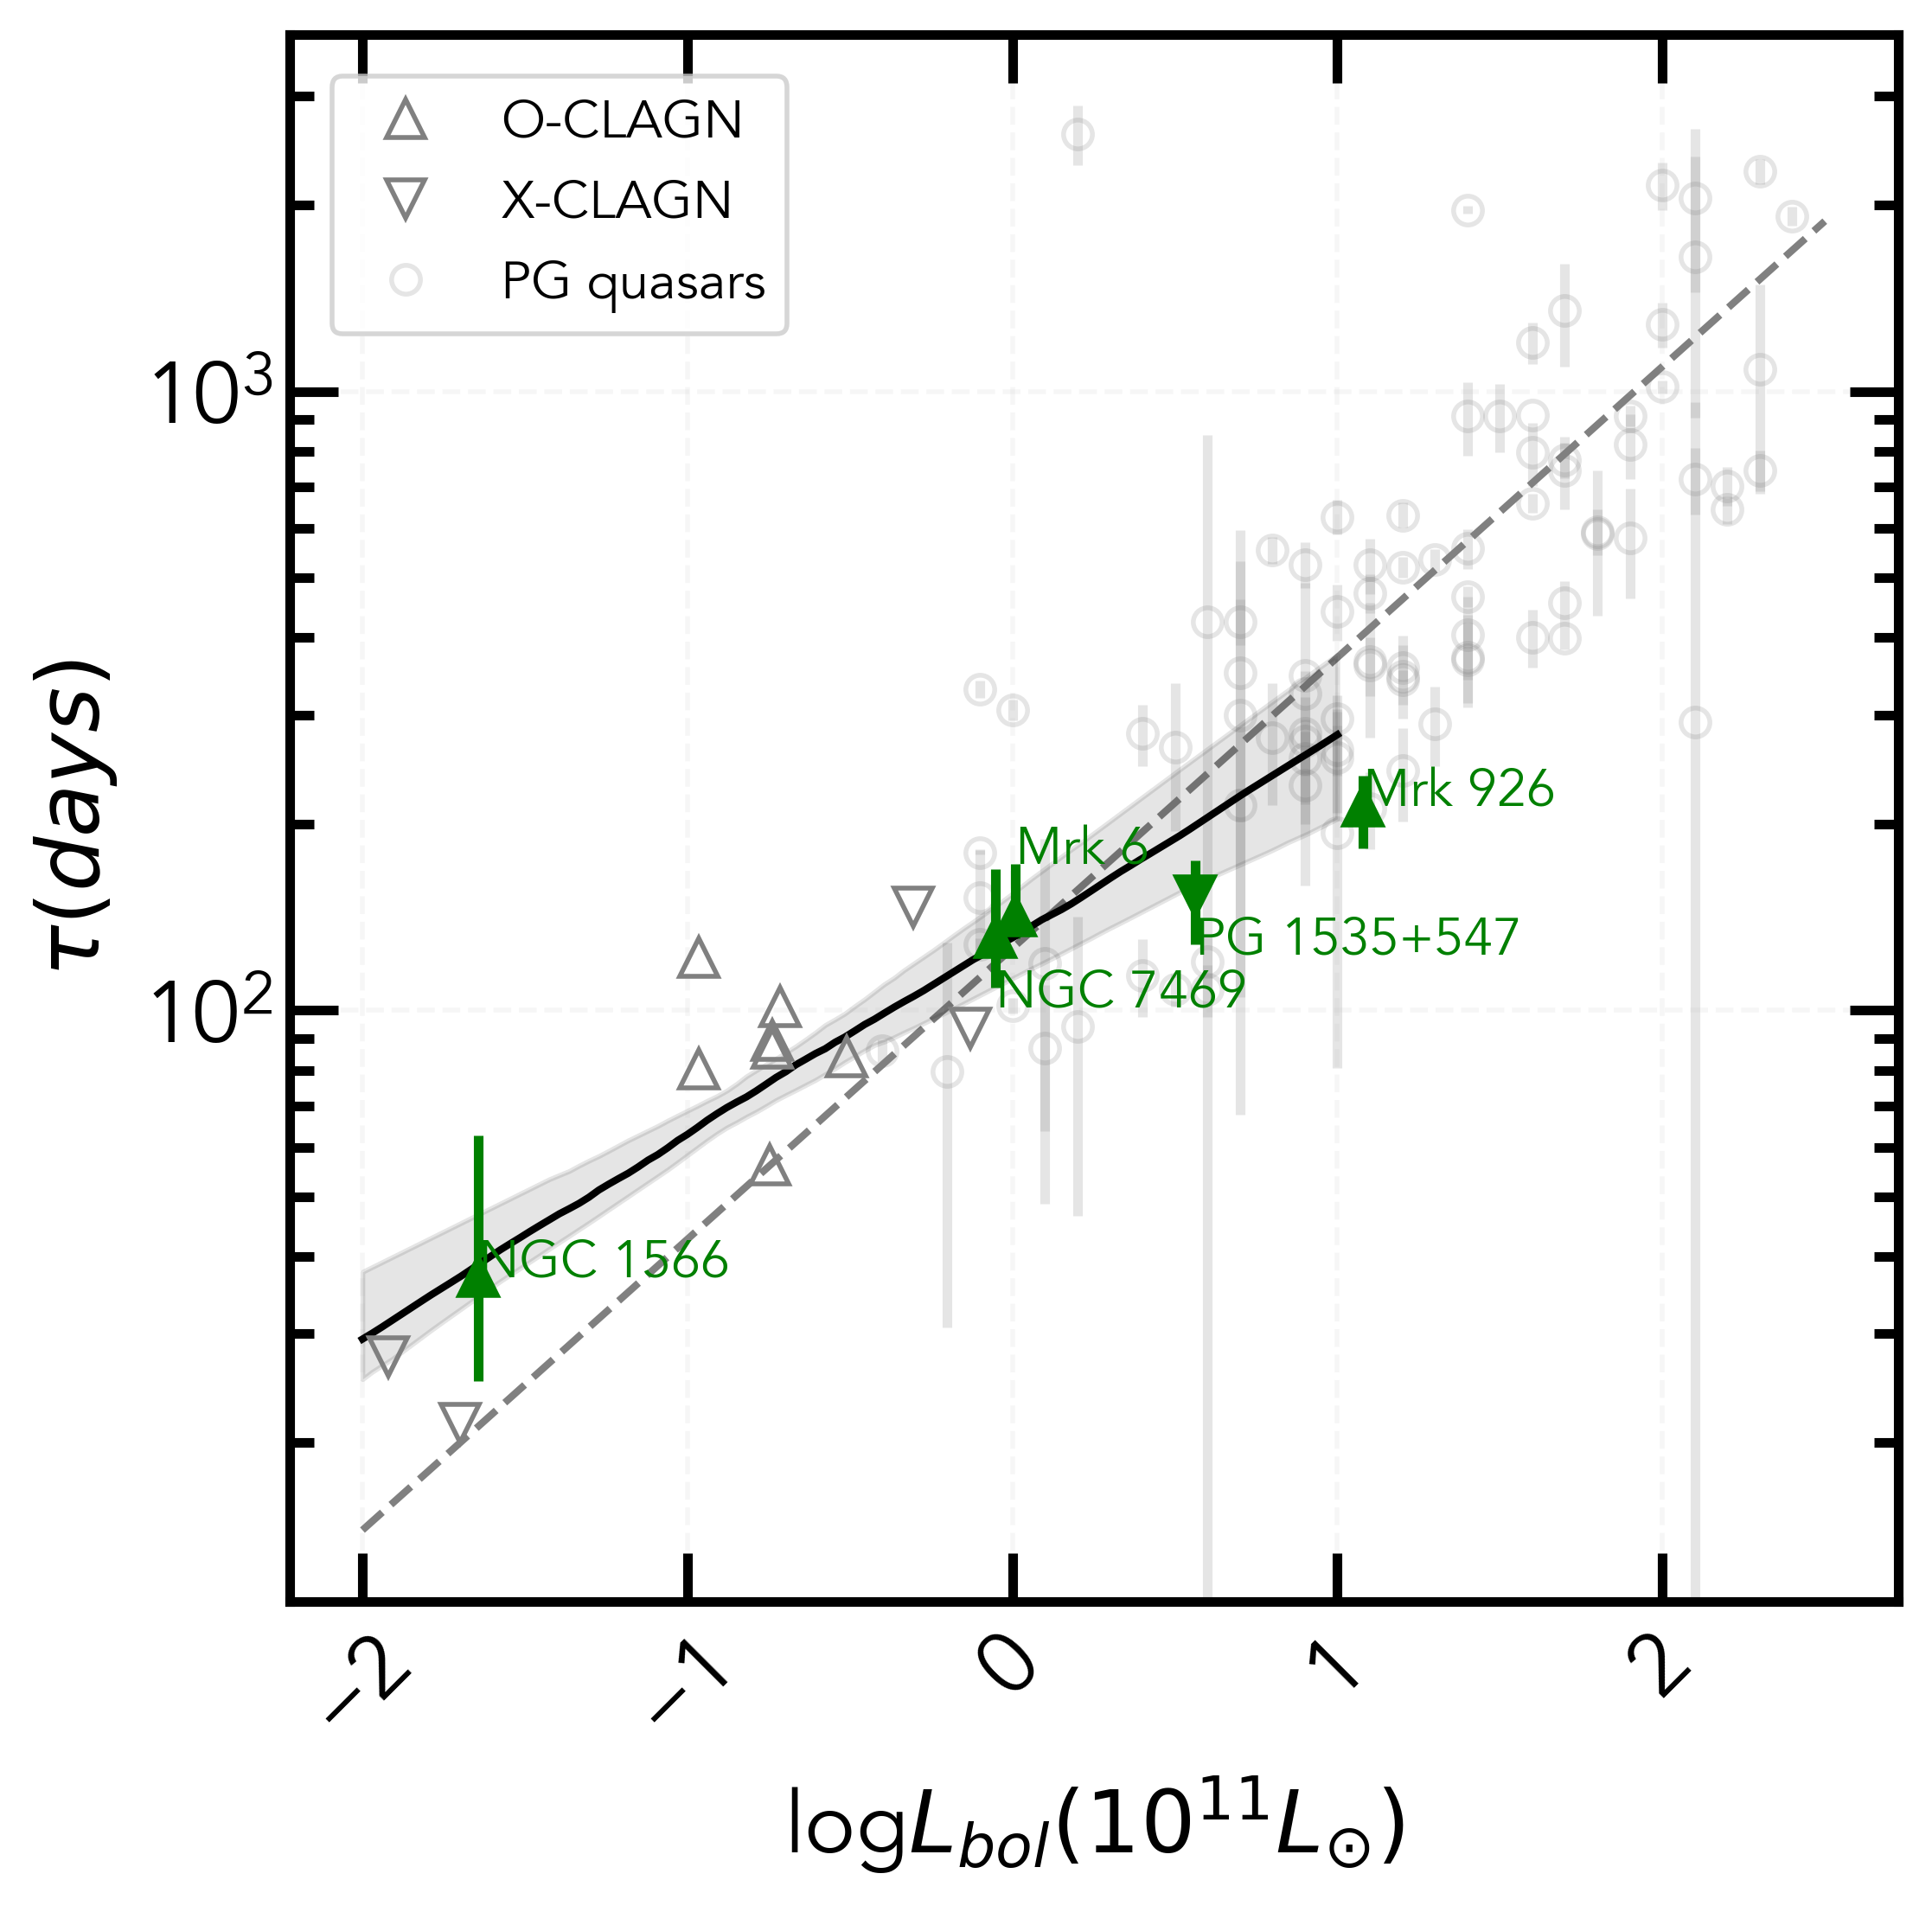
\includegraphics[width=0.5\textwidth]{tau_L_correlation_clagn.png}
    \caption{$\tau$-L correlation for CLAGNs, where $\tau$ is time lag between V band and $W$1 band and L is bolometric luminosity. Grey circles represent PG quasars \citep{2019ApJ...886...33L} for comparison. The dashed line repserent the best fitting of $\tau$-L correlation for PG quasars in \citet{2019ApJ...886...33L}.  The solid triangles are results in this work, while the open triangles are results from \citet{2014ApJ...788..159K} and \citet{2019ApJ...886...33L}. The straight line is the best fitting for CLAGNs with a scatter of 0.14 in the shadow region.} 
    \label{fig:tau_L}
\end{figure}


\begin{table}
 \caption{Dust reverberation time lag of CLAGNs.
}
 \label{table_lag}
 \begin{center}
 \begin{tabular}{lccccc}
 \hline\hline
Name & log($L_{bol}/L_{\odot}$) & $\tau$~(days) &Type  & references\\ \hline 
NGC 1566 & 9.36 & $37.1^{+25.7}_{-11.9}$ & O & This work \\
Mrk 6 & 11.01 & $142.1^{+30.0}_{-11.5}$ & O & This work \\
Mrk 926 & 12.08 & $213.8^{+25.3}_{-31.0}$ & O & This work \\
PG 1535+547 & 11.56 & $153.2^{+21.2}_{-25.3}$ & X & This work \\
NGC 7469 & 10.95 & $131.2^{+37.9}_{-22.4}$ & O & This work \\
Mrk 590 & 10.25 & $ 33.8 \pm 4.20$ & O & \citet{2014ApJ...788..159K} \\
NGC 3516 & 10.03 & $ 73.1 \pm 4.00$ & O & \citet{2014ApJ...788..159K} \\
NGC 4051 & 9.08 & $ 16.5 \pm 0.60$ & X & \citet{2014ApJ...788..159K} \\
NGC 4151 & 10.03 & $ 48.3 \pm 0.50$ & O & \citet{2014ApJ...788..159K} \\
NGC 5548 & 10.29 & $ 60.9 \pm 0.30$ & O & \citet{2014ApJ...788..159K} \\
NGC 7469 & 10.69 & $ 88.0 \pm 0.60$ & X & \citet{2014ApJ...788..159K} \\
NGC 3516 & 10.26 & 53.6 & O & \citet{2019ApJ...886...33L} \\
NGC 4051 & 9.30 & 12.9 & X & \citet{2019ApJ...886...33L} \\
NGC 4151 & 10.26 & 52.2 & O & \citet{2019ApJ...886...33L} \\
NGC 5548 & 10.49 & 50.5 & O & \citet{2019ApJ...886...33L} \\
NGC 7469 & 10.87 & 56.1 & X & \citet{2019ApJ...886...33L} \\
\hline\hline
\end{tabular}
\end{center}
Note. The table lists source name, bolometric luminosity, dust reverberation time lag, CLAGN types (``O'' for optical selected CLAGN and ``X'' for X-ray selected CLAGN) and references. The time lags estimated in this work are between V band and $W$1 band. The time lag results from \citet{2014ApJ...788..159K} and \citet{2019ApJ...886...33L} are between V band and K band, which are scaled to $\tau_\mathrm{W1}$ with $\tau_\mathrm{W1}=\tau_\mathrm{K} \times \frac{5}{3}$ in the $\tau$-$L_{bol}$ correlation of \autoref{fig:tau_L}. 
\end{table}

%The time lag for NGC 2617 is between \uvot\, UVW2 ($\sim 1928\,\AA$)  and K band ($\sim 2.19\,\mu$m).
%Also, to avoid a spurious peaks at ∼15 days, the spacing between the distinct two peaks visible in light curves, we forced JAVELIN to only return lags of <10 days\citet{2014ApJ...788...48S}.